\newpage
\chapter{PENDAHULUAN} \label{Bab I}

\section{Latar Belakang} \label{I.Latar Belakang}
Komunikasi adalah fondasi utama dalam membangun interaksi sosial manusia. Melalui komunikasi, seseorang dapat menyampaikan informasi, membangun pemahaman, dan menjalin hubungan yang harmonis dengan lingkungan sekitar. Namun, bagi penyandang tunarungu, kegiatan sederhana ini justru menjadi tantangan tersendiri. Hambatannya bukan terletak pada ketidakmampuan mereka memahami bahasa tulisan, melainkan pada kenyataan bahwa sebagian besar masyarakat umum belum memahami bahasa isyarat sebagai sarana komunikasi utama komunitas Tuli.\par

\begin{figure}[H] % Kalau menggunakan H, posisi gambar akan tepat dibawah teks
    \centering
    \fbox{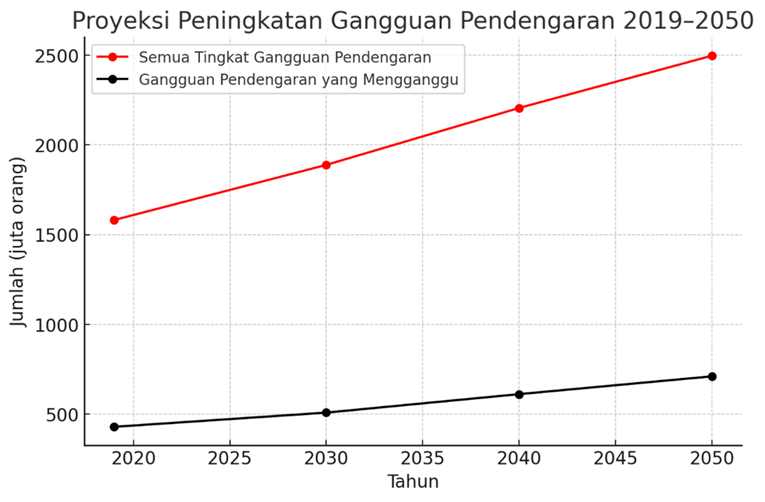
\includegraphics[width=0.8\textwidth]{figure/proyeksi.png}}
    \caption[Proyeksi WHO 2019–2050 populasi dengan gangguan pendengaran]{Proyeksi WHO 2019–2050 populasi dengan gangguan pendengaran \cite{WorldHealthOrganizationWHO2021}}
    \label{fig:1.proyeksi}
\end{figure}

Skala permasalahan ini cukup besar jika dilihat dari data global. World Health Organization (WHO) melaporkan bahwa pada tahun 2019 terdapat lebih dari 1.57 miliar orang di dunia yang hidup dengan gangguan pendengaran, dan sekitar 430 juta di antaranya tergolong mengalami gangguan tingkat sedang hingga berat (\textit{disabling hearing loss}). Proyeksi WHO pada Gambar~\ref{fig:1.proyeksi} menunjukkan bahwa angka tersebut diperkirakan terus meningkat hingga mencapai sekitar 2.5 miliar jiwa pada tahun 2050, dengan lebih dari 700 juta orang diperkirakan membutuhkan rehabilitasi pendengaran \cite{WorldHealthOrganizationWHO2021}. Tren kenaikan ini menegaskan bahwa gangguan pendengaran bukan sekadar persoalan individu, melainkan isu global yang membutuhkan dukungan teknologi untuk mengatasi hambatan komunikasi yang muncul dari keterbatasan pendengaran.\par

Situasi serupa juga terjadi di Indonesia. Badan Pusat Statistik (BPS) melalui publikasi \textit{Potret Penyandang Disabilitas di Indonesia: Hasil Long Form SP2020} mencatat terdapat 933.893 penyandang disabilitas, dan 17.12\% atau 159.918 jiwa di antaranya termasuk kategori keterbatasan sensorik seperti rungu dan netra \cite{BadanPusatStatistikBPS2024}. Data Dataloka.id yang mengutip hasil Susenas 2022 juga memperlihatkan bahwa kelompok ini masih menghadapi kesenjangan akses terhadap komunikasi dan pendidikan \cite{Datalokaid2023}. Di sisi lain, tren pendidikan inklusif mendorong semakin banyak siswa dengan keterbatasan sensorik bersekolah di sekolah umum, padahal guru dan siswa lain umumnya belum menguasai bahasa isyarat. Akibatnya, hambatan komunikasi justru kerap terjadi di lingkungan belajar yang seharusnya menjadi ruang paling mendukung bagi mereka \cite{Ratriyana2022}.\par

Hambatan tersebut tidak berhenti di ruang kelas. Dalam layanan kesehatan, tenaga medis sering kesulitan memahami keluhan pasien tunarungu karena ketiadaan penerjemah bahasa isyarat. Dalam interaksi sehari-hari, baik di tempat kerja maupun fasilitas publik, penyandang tunarungu juga kerap kesulitan menyampaikan maksudnya, yang pada akhirnya mendorong isolasi sosial dan keterbatasan partisipasi dalam kehidupan masyarakat \cite{Tannenbaum-Baruchi2025}.\par

Bahasa isyarat menjadi solusi utama untuk menjembatani hambatan tersebut. Di Indonesia dikenal dua sistem bahasa isyarat utama, yaitu Bahasa Isyarat Indonesia (BISINDO) dan Sistem Isyarat Bahasa Indonesia (SIBI). BISINDO tumbuh secara alami di komunitas Tuli sehingga bersifat idiomatik dan ekspresif, sedangkan SIBI merupakan sistem isyarat baku yang distandardisasi oleh pemerintah untuk keperluan pendidikan formal karena mengikuti tata bahasa Indonesia \cite{Ratriyana2022,Zulpicha2017}. Salah satu ciri khas SIBI adalah penggunaan imbuhan yang direpresentasikan secara eksplisit pada kata dasar. Kata ``membaca'', misalnya, terbentuk dari imbuhan ``me-'' dan kata dasar ``baca''. Struktur linguistik yang konsisten inilah yang membuat SIBI relatif lebih mudah dipetakan ke dalam sistem penerjemahan otomatis berbasis komputer \cite{RakunWidhinugraha2022}.\par


Keterbatasan jumlah penerjemah manusia menjadikan sistem penerjemah bahasa isyarat berbasis teknologi sebagai kebutuhan yang semakin mendesak. Penelitian terdahulu telah mengeksplorasi beragam pendekatan \textit{Computer Vision} dan \textit{Deep Learning} untuk mengenali SIBI, mulai dari penggabungan fitur kerangka tubuh dan bentuk tangan (\textit{skeletal features}) \cite{RakunSetyono2022}, pemanfaatan \textit{transfer learning} pada CNN \cite{Pratama2025}, hingga penggunaan arsitektur \textit{Transformer} untuk penerjemahan berbasis teks \cite{Aurelrius2025}. Pendekatan yang berfokus pada ekstraksi fitur skeletal (seperti MediaPipe) sering digunakan karena komputasinya yang ringan. Namun, ekstraksi fitur rangka ini memiliki kelemahan mendasar untuk domain bahasa isyarat. Pertama, algoritma pendeteksi titik kunci (\textit{keypoint estimation}) sangat rentan terhadap oklusi diri (\textit{self-occlusion}), misalnya ketika jari saling menutupi, kedua tangan bersilangan, atau bergerak sangat cepat, yang merupakan kondisi lazim dalam SIBI. Kegagalan deteksi pada tahap ekstraksi awal ini akan terakumulasi dan secara langsung membatasi tingkat akurasi model klasifikasi akhir. Kedua, representasi abstrak berupa koordinat kerangka membuang sebagian besar informasi visual yang berharga, seperti tekstur, bentuk rinci permukaan tangan, perubahan orientasi telapak tangan secara 3D, serta konteks interaksi antara tangan dan tubuh penanda isyarat \cite{Li2020WLASL}.\par

Oleh karena itu, penelitian ini memilih untuk tidak menggunakan fitur skeletal, melainkan memproses data video mentah (\textit{raw RGB}) secara langsung (\textit{end-to-end}) \cite{Tong2022VideoMAE, Carreira2017I3D}. Dengan memanfaatkan video \textit{raw RGB}, model dapat mempelajari representasi rupa (\textit{appearance}) sekaligus dinamika gerak (\textit{motion}) secara simultan dari kumpulan piksel asli tanpa bergantung pada ketepatan algoritma ekstraksi fitur pihak ketiga. Detail halus yang membedakan isyarat bermakna mirip tetap dipertahankan, sehingga model dapat menangkap relasi spasio-temporal yang komprehensif. Meski begitu, memproses video \textit{raw RGB} menuntut penggunaan arsitektur pemahaman video yang jauh lebih canggih untuk mengatasi tingginya kompleksitas data dibandingkan modul rekuren konvensional yang sering dipakai pada fitur statis.\par

Di sisi lain, perkembangan arsitektur pemahaman video membuka peluang untuk mengatasi keterbatasan pendekatan terdahulu yang umumnya masih bergantung pada ekstraksi fitur manual atau modul rekuren konvensional. Dua arsitektur yang menjadi model pembanding dalam penelitian ini adalah \textit{I3D} (\textit{Inflated 3D ConvNets}) dan \textit{Video Vision Transformer} (ViViT). I3D yang diperkenalkan Carreira dan Zisserman \cite{Carreira2017I3D} bekerja dengan mengembangkan filter 2D pra-latih menjadi 3D sehingga mampu mempelajari representasi spasio-temporal secara \textit{end-to-end} tanpa kehilangan manfaat bobot pra-latih dari domain citra, dan telah terbukti sebagai \textit{baseline} baku pada berbagai tugas pengenalan aksi maupun bahasa isyarat berbasis video. Sementara itu, ViViT yang diperkenalkan oleh Arnab dkk.\ \cite{Arnab2021} merupakan arsitektur berbasis Transformer murni yang memproses video sebagai barisan token spasio-temporal dan mengandalkan \textit{self-attention} untuk memodelkan hubungan ruang-waktu tanpa komponen konvolusi sama sekali, dilatih secara \textit{supervised} pada dataset video berskala besar.\par

Sebagai model utama, penelitian ini memilih \textit{VideoMAE} (\textit{Video Masked Autoencoder}). VideoMAE mengadopsi paradigma \textit{self-supervised} dengan menerapkan \textit{tube masking} ekstrem hingga 90--95\% pada token spasio-temporal video, sehingga model dipaksa merekonstruksi informasi yang tertutup dan dengan demikian membangun representasi spasio-temporal yang kuat tanpa memerlukan label anotasi dalam jumlah besar \cite{Tong2022VideoMAE}. Sifat \textit{data-efficient} inilah yang mendasari pemilihannya sebagai model utama, mengingat dataset SIBI yang digunakan dalam penelitian ini tergolong kecil. Relevansi pendekatan ini pada domain bahasa isyarat juga telah dibuktikan secara empiris oleh Alsraisri \cite{Alsraisri2025}, yang menerapkan VideoMAE pada \textit{Arabic Sign Language Recognition} dan berhasil mencapai akurasi \textit{state-of-the-art}, sehingga memberikan landasan kuat bahwa paradigma ini layak diadaptasi ke konteks SIBI.\par

Ketiga model tersebut masing-masing mewakili paradigma pemodelan video yang berbeda: I3D mewakili pendekatan 3D CNN \textit{supervised} yang mengandalkan konvolusi lokal untuk menangkap dinamika temporal, ViViT mewakili \textit{supervised video transformer} yang memodelkan relasi global antar-token tanpa konvolusi, dan VideoMAE mewakili \textit{self-supervised video transformer} yang memanfaatkan rekonstruksi termasking untuk memperoleh representasi yang \textit{data-efficient}. Dengan menempatkan VideoMAE sebagai model utama dan I3D serta ViViT sebagai pembanding, penelitian ini tidak hanya bertujuan mengidentifikasi model yang paling unggul pada data SIBI terkontrol, tetapi juga memberikan dasar empiris mengenai keunggulan masing-masing paradigma dalam konteks pengenalan bahasa isyarat Indonesia.\par

Berdasarkan pertimbangan tersebut, penelitian ini menggunakan VideoMAE sebagai model utama untuk klasifikasi gerakan visual Bahasa Isyarat SIBI, dengan I3D dan ViViT sebagai model pembanding. Perbandingan ini tidak dimaksudkan sekadar menghadapkan tiga arsitektur, melainkan untuk menguji tiga paradigma sekaligus: 3D CNN \textit{supervised} (I3D) yang telah terbukti pada bahasa isyarat, \textit{supervised video transformer} (ViViT) yang mewakili arsitektur Transformer murni untuk video, dan \textit{self-supervised video transformer} (VideoMAE) yang menunjukkan keberhasilan pada Arabic Sign Language. Dengan demikian, hasil penelitian diharapkan tidak hanya menjawab model mana yang lebih unggul pada data SIBI terkontrol, tetapi juga memberikan dasar empiris mengenai keunggulan masing-masing paradigma pemodelan video dalam konteks pengenalan bahasa isyarat Indonesia.\par


\section{Rumusan Masalah} \label{I.Rumusan Masalah}
Berdasarkan uraian latar belakang di atas, permasalahan yang diangkat dalam penelitian ini berfokus pada analisis kinerja model \textit{VideoMAE} dalam melakukan klasifikasi gerakan visual Bahasa Isyarat SIBI, serta perbandingan hasil klasifikasinya dengan model \textit{I3D} dan \textit{ViViT} sebagai model pembanding berdasarkan akurasi dan \textit{confusion matrix}.\par


\section{Tujuan Penelitian} \label{I.Tujuan}
Penelitian ini bertujuan menerapkan dan menganalisis kinerja model VideoMAE dalam mengenali dan mengklasifikasikan gerakan visual Bahasa Isyarat SIBI. Selain itu, penelitian ini juga membandingkan hasil klasifikasi VideoMAE dengan I3D dan ViViT sebagai model pembanding menggunakan akurasi dan \textit{confusion matrix} sebagai metrik evaluasi.\par

\section{Batasan Masalah} \label{I.Batasan}
Agar penelitian ini tetap terarah dan dapat diselesaikan secara realistis, ditetapkan sejumlah batasan masalah sebagai berikut:

\begin{enumerate}
    \item Penelitian ini berfokus pada klasifikasi kata terisolasi (\textit{isolated word recognition}) Bahasa Isyarat Indonesia (SIBI), yaitu setiap klip video berisi satu kata dasar yang dilakukan secara terpisah. Penelitian ini tidak mencakup pengenalan kalimat kontinu (\textit{continuous sign language recognition}) maupun deteksi segmentasi batas kata antar isyarat.

    \item Modalitas yang digunakan terbatas pada data video (visual), tanpa melibatkan audio, teks, data sensor gerak (\textit{IMU}/\textit{depth}), maupun modalitas non-manual lainnya seperti ekspresi wajah dan gerak bibir.

    \item Cakupan kosakata dibatasi pada 10 kata dasar SIBI (aku, bapak, bawa, guru, ibu, kamu, mau, pulang, sekolah, suka) yang dipilih berdasarkan observasi awal sebagai kosakata yang paling sering digunakan dalam komunikasi sehari-hari di lingkungan sekolah. Generalisasi terhadap kosakata lain di luar daftar ini tidak dicakup dalam penelitian ini.

    \item Dataset SIBI yang digunakan merupakan hasil perekaman dalam kondisi terkontrol, yaitu ruangan tertutup dengan pencahayaan stabil, latar belakang polos, dan jarak kamera yang tetap. Kinerja model pada kondisi dunia nyata yang tidak terkontrol (variasi pencahayaan, latar kompleks, sudut pandang berbeda) tidak dievaluasi.

    \item Model VideoMAE dianalisis pada dua variasi sumber pra-latih yang tersedia secara publik, yaitu Kinetics-400 dan Something-Something V2. Bobot pra-latih digunakan apa adanya tanpa modifikasi pada tahap pra-latih ulang (\textit{pre-training from scratch} pada domain lain).

    \item Konfigurasi model pembanding (ViViT dan I3D) menggunakan hyperparameter standar yang ditentukan berdasarkan praktik umum pada literatur; penelitian ini tidak melakukan pencarian \textit{hyperparameter} yang ekstensif untuk model pembanding tersebut.

    \item Evaluasi performa difokuskan pada metrik akurasi validasi (\textit{Best Val Acc@1}), \textit{Macro F1-score}, \textit{Mean Absolute Error} (MAE), serta analisis \textit{confusion matrix} dan laporan klasifikasi per kelas. Waktu inferensi diukur secara terbatas sebagai analisis kelayakan \textit{deployment}, namun metrik efisiensi komputasi lainnya seperti waktu pelatihan, \textit{throughput}, dan konsumsi daya tidak dievaluasi.

    \item Penelitian ini hanya mencakup tahap analisis kinerja dan perbandingan hasil klasifikasi, tanpa mengembangkan sistem penerjemah bahasa isyarat berbasis \textit{real-time} maupun aplikasi untuk pengguna akhir (\textit{end-user}).
\end{enumerate}

\section{Manfaat Penelitian} \label{I.Manfaat}
Hasil penelitian ini diharapkan dapat memberikan manfaat sebagai berikut:

\begin{enumerate}
    \item Bagi pengembangan teknologi, penelitian ini diharapkan dapat menjadi dasar empiris dalam pemanfaatan model \textit{self-supervised video transformer} seperti VideoMAE untuk klasifikasi gerakan bahasa isyarat di Indonesia.
    \item Bagi akademisi dan peneliti, penelitian ini diharapkan dapat menjadi referensi mengenai pengaruh perbedaan dataset \textit{pre-training} terhadap performa model dalam tugas pengenalan gerakan visual.
    \item Bagi komunitas Tuli, penelitian ini diharapkan dapat memberikan kontribusi awal dalam pengembangan sistem pengenalan bahasa isyarat berbasis video yang mendukung interaksi yang lebih inklusif di masa depan.
\end{enumerate}

\section{Sistematika Penulisan} \label{I.Sistematika}
Laporan Tugas Akhir ini disusun secara sistematis ke dalam lima bab yang saling berkaitan agar alur penelitian tersaji secara logis dan komprehensif.\par

\subsection{Bab I Pendahuluan}
Bab ini berfungsi sebagai fondasi penelitian. Pembahasan dimulai dari latar belakang masalah yang memaparkan urgensi dan relevansi topik, dilanjutkan dengan rumusan masalah, tujuan penelitian, batasan masalah, manfaat penelitian, serta gambaran umum struktur laporan yang akan disajikan pada bab-bab berikutnya.\par

\subsection{Bab II Tinjauan Pustaka}
Bab ini membangun kerangka teoretis dan kontekstual bagi penelitian. Pembahasan mencakup tinjauan kritis terhadap penelitian terdahulu di bidang pengenalan bahasa isyarat, khususnya SIBI, untuk mengidentifikasi celah penelitian. Selain itu, dijabarkan pula landasan teori yang digunakan, meliputi konsep Sistem Isyarat Bahasa Indonesia (SIBI), \textit{computer vision}, arsitektur \textit{Video Transformer}, konsep \textit{Masked Autoencoder} (MAE), serta metrik evaluasi kinerja model seperti akurasi, \textit{precision}, \textit{recall}, dan \textit{F1-score}.\par

\subsection{Bab III Metode Penelitian}
Bab ini menguraikan rancangan dan langkah-langkah metodologis yang ditempuh dalam penelitian. Pembahasan dimulai dari alur penelitian secara keseluruhan, proses pengumpulan data video, teknik pra-pemrosesan data visual, hingga perancangan arsitektur model VideoMAE. Prosedur pelatihan, validasi, dan pengujian model beserta metrik evaluasi yang digunakan juga dijelaskan secara rinci.\par

\subsection{Bab IV Hasil dan Pembahasan}
Bab ini merupakan inti penyajian temuan penelitian. Hasil pengujian model dipaparkan secara kuantitatif dan kualitatif dalam enam kelompok eksperimen: (1) perbandingan \textit{backbone} dan dataset \textit{pre-train}, (2) strategi pelatihan \textit{pre-train} versus \textit{scratch}, (3) strategi \textit{sampling} frame, (4) pengaruh jumlah \textit{epoch}, (5) pengaruh augmentasi \textit{mixup}/\textit{CutMix}/\textit{reprob}, dan (6) perbandingan lintas arsitektur antara VideoMAE, ViViT, dan I3D. Setiap kelompok dianalisis menggunakan kurva pelatihan, \textit{confusion matrix}, dan laporan klasifikasi per kelas. Bab ini juga menyajikan analisis waktu inferensi sebagai kajian kelayakan \textit{deployment} dari masing-masing model.\par

\subsection{Bab V Kesimpulan dan Saran}
Bab ini menjadi penutup laporan penelitian. Kesimpulan yang ditarik dari hasil analisis dan pembahasan dirangkum untuk menjawab rumusan masalah yang telah ditetapkan. Berdasarkan temuan dan keterbatasan yang ditemukan, diajukan pula saran-saran konstruktif bagi pengembangan penelitian selanjutnya maupun potensi penerapan praktis dari sistem pengenalan bahasa isyarat berbasis \textit{video transformer}.\par
